\subsection{Recovery of the Schwarzschild Metric}
  \label{subsec:recovery-of-the-schwarzschild-metric}

  In the presence of a static and approximately spherically symmetric distribution of
  localized projected configurations, the collective reduction of admissible relaxation
  ordering admits a simple effective description.
  In the weak-constraint and quasi-static regime, spatial variations of the effective
  ordering rate can be summarized by a Poisson-like relation between an effective
  gravitational potential and the density of localized projected configurations.

  When expressed in an effective geometric language, this structure is well described
  by a metric whose leading-order form coincides with the Schwarzschild solution of
  general relativity.
  In particular, the temporal and radial components of the effective metric encode the
  local reduction of admissible relaxation ordering induced by a localized projected
  configuration, while the angular sector reflects the approximate isotropy of the
  effective description.

  Within this framework, standard weak-field predictions of general relativity are
  recovered.
  These include gravitational redshift, light deflection, and time dilation effects
  consistent with solar-system observations.
  The gravitational constant $G$ appears as an emergent coupling parameter relating the
  effective density of localized projected configurations to the magnitude of the
  ordering slowdown.

  \begin{figure}[htbp]
    \centering
    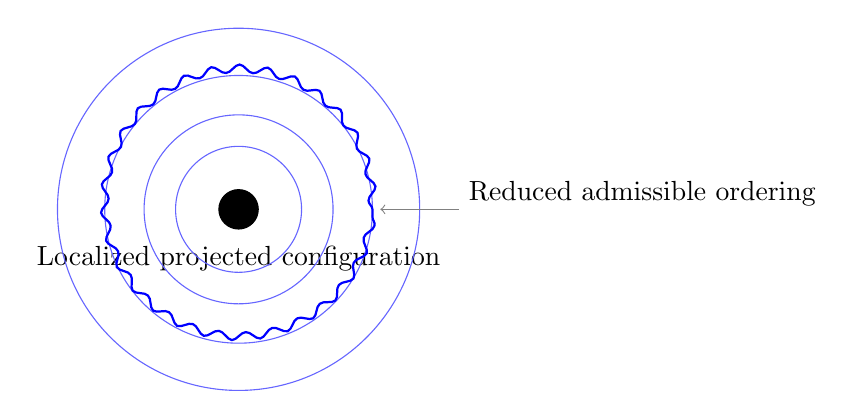
\begin{tikzpicture}[scale=1]

% Central mass
      \filldraw[black] (0,0) circle (0.25);
      \node[below] at (0,-0.35) {Localized projected configuration};

% Effective ordering contours
      \foreach \r in {0.8,1.2,1.7,2.3} {
        \draw[blue!60] (0,0) circle (\r);
      }

% Distortion
      \draw[blue, thick, decorate, decoration={snake, amplitude=0.5mm}]
      (0,0) circle (1.7);

% Arrows
      \draw[->, gray] (2.8,0) -- (1.8,0);
      \node[right] at (2.8,0.2) {Reduced admissible ordering};

    \end{tikzpicture}
    \caption
    {Emergence of Schwarzschild-like behavior in Cosmochrony.
    A localized projected configuration induces a spatially varying reduction of
    admissible relaxation ordering.
    In effective geometric descriptions, this manifests as differential proper-time
    flow and an emergent metric curvature analogous to gravitational time dilation.}
    \label{fig:chi_gravity}
  \end{figure}

  Importantly, the Schwarzschild metric is not postulated as a fundamental solution,
  nor is spacetime curvature treated as a primitive entity.
  Rather, the metric provides a compact and effective summary of how localized projected
  configurations constrain admissible relaxation ordering in their vicinity.

  In this sense, Schwarzschild-like behavior does not reflect a specific dynamical law
  of spacetime itself, but emerges as the necessary phenomenological description in
  regimes where projected configurations are close to local equilibrium and admit a
  geometric interpretation.
